\section{User Stories}
	\subsection{Personas}
		\begin{description}
			\item[Olivia Zander]\label{olivia}\ \newline
				\begin{minipage}[t]{0.35\textwidth} 
					\begin{figure}[H]
						\vspace{-0.75cm}
						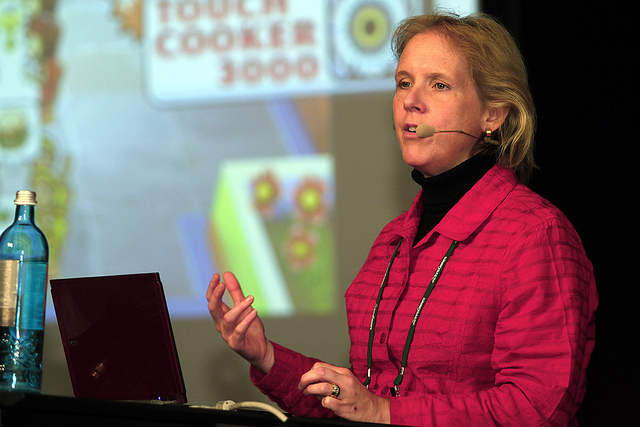
\includegraphics[trim=0cm 0cm 0cm 0cm, clip=true, width=5cm]{requirements/media/img/oliviaZander.jpg}
						\caption[Symbolbild Persona Olivia Zander\newline 
							\license{CC BY 2.0 \url{https://creativecommons.org/licenses/by/2.0/}  Official GDC \url{https://www.flickr.com/photos/officialgdc/}}
						]
						{\label{Olivia Zander}}
					\end{figure}
				\end{minipage}
				\begin{minipage}[t]{0.55\textwidth}
					52 Jahre alt.
					Olivia ist eine erfahrene \textbf{Softwarearchitekt}in und arbeitet schon viele Jahre auf dem Beruf.
					Aktuell arbeitet sie in einem kleinen Beratungsunternehmen, welches andere Firmen beim Umstrukturieren von Softwareapplikationen unterstützt.
					Vor einiger Zeit hat sie eine Weiterbildung im Bereich Cloud Computing gemacht.
					Seither hat sie selbst Erfahrungen damit sammeln können, nämlich in verschiedene Beratungsprojekten in welchen es darum ging, bestehende Anwendungen in die Cloud zu bringen.
				\end{minipage}
			\item[Thomas Bucher]\label{thomas}\ \newline
				\begin{minipage}[t]{0.35\textwidth} 
					\begin{figure}[H]
						\vspace{-0.75cm}
						
\includegraphics[trim=0cm 0cm 0cm 0cm, clip=true, width=5cm]{requirements/media/img/thomasBucher.jpg}
						\caption[Symbolbild Persona Thomas Bucher\newline
							\license{CC BY 2.0 \url{https://creativecommons.org/licenses/by/2.0/} Steve wilson \url{https://www.flickr.com/photos/125303894@N06/}}
						]
						{\label{Thomas Bucher}}
					\end{figure}
				\end{minipage}
				\begin{minipage}[t]{0.55\textwidth}
					29 Jahre alt.
					Thomas hat vor ein paar Jahren in Rapperswil den Informatik-Bachelor abgeschlossen und arbeitet seither in der gleichen Firma wie Olivia.
					Er arbeitet da als \textbf{Projektplaner} und unterstützt in dieser Funktion aktuell eine externe Firma eine Anwendung mit täglich rund 10'000 Benutzern von ihren lokalen Servern in die Cloud zu transferieren.
				\end{minipage}
		\end{description}
		
	\subsection{Definitionen}\label{userstoryDefinitions}
		Folgende Wörter werden in den User Stories verwendet und sind dafür zum genauen Verständnis hier definiert.
		\begin{description}
			\item[Wissensproduzent] Person, die neues Wissen ins System (\cdar\ und \eeppi) einpflegt (als Beispiel kann hier \hyperref[olivia]{Olivia} dienen).
			\item[Problem space (Wissensbaum im \cdar)] Ein Projekt im \cdar\, in welchem ein Wissensproduzent Wissen ablegt.
			\item[Wissenskonsument] Person, die einen Problem space benutzt um damit Entscheide zu fällen (als Beispiel kann hier \hyperref[thomas]{Thomas} dienen).
			\item[Solution space (Entscheidungsprojekt im \cdar)] Ein Projekt im \cdar\, aus welchem ein Wissenskonsument Wissen konsumiert.
				Es ist jeweils eine Kopie eines Wissensbaums.
			\item[Administrator] Person, die für die Konfiguration und den Betrieb von \eeppi\ verantwortlich ist.
			\item[Abbildung] Mit einer Abbildung lässt sich ein Datensatz in einen anderen Datensatz umwandeln.
			\item[erstellen aus] Als Grundlage wird ein Datensatz genommen, aus welchem ein neuer Datensatz erstellt wird.
				Anschliessend sind die beiden Datensätze voneinander unabhängig und Änderungen an einem Datensatz beeinflussen den anderen Datensatz nicht.
			\item[Task] Datensatz, welcher eine Aufgabe beschreibt.
			% Task-Vorlage, Entscheidungs-Vorlage: Wortwahl gemäss Duden Regel 22
			\item[Task-Vorlage] Datensatz, um später daraus Tasks in einem \ppt\ zu erstellen.
			\item[Entscheidungs-Task] Task, welcher zum Treffen einer Entscheidung erledigt werden muss.
				Er ist einem Problem/Solution space item angehängt.
			\item[Operativer Task] Task, welcher durch das Treffen einer Option entsteht.
				Er ist dementsprechend einer Option angehängt.
			\item[Problem space item] Datensatz, der eine Wahl mit mehreren Optionen darstellt.
				Der Datensatz ist jedoch nur eine Vorlage, die Entscheidung kann nicht getroffen werden
			\item[Solution space item] Datensatz, der eine Wahl mit mehreren Optionen darstellt.
				Er wird aus einer Entscheidungs-Vorlage erstellt.
				Die Entscheidung kann jetzt getroffen werden.
			\item[Entscheid] Getroffenes (entschiedenes) Solution space item.
			\item[Option] Möglichkeit, wie eine Entscheidung entschieden wird.
			\item[entscheiden] Tätigkeit, in welcher für ein Solution space item der Entscheid gefällt wird.
			\item[importieren] Anwenden einer Abbildung zur Aufnahme von Datensätzen in das \eeppi.
			\item[exportieren] Anwenden einer Abbildung zur Ausgabe von Datensätzen aus dem \eeppi.
			\item[\ppt] Externes Programm, welches Tasks verwaltet und für diese Tasks eine eigene Form erwartet.
			\item[API] Schnittstelle eines Programms (sowohl bei externen, als auch \cdar\ und \eeppi)
		\end{description}

		
	\begin{landscape}
	\subsection{Übersicht über die User Stories}
	
		\eeppi\ hat eine enge Verbindung zu \cdar\ und deshalb werden in Abbildung~\ref{fig:UserStoryDiagram} auch in einem ersten Schritt gemeinsam die übergeordneten User Stories beschrieben.
	
		\begin{figure}[H]
				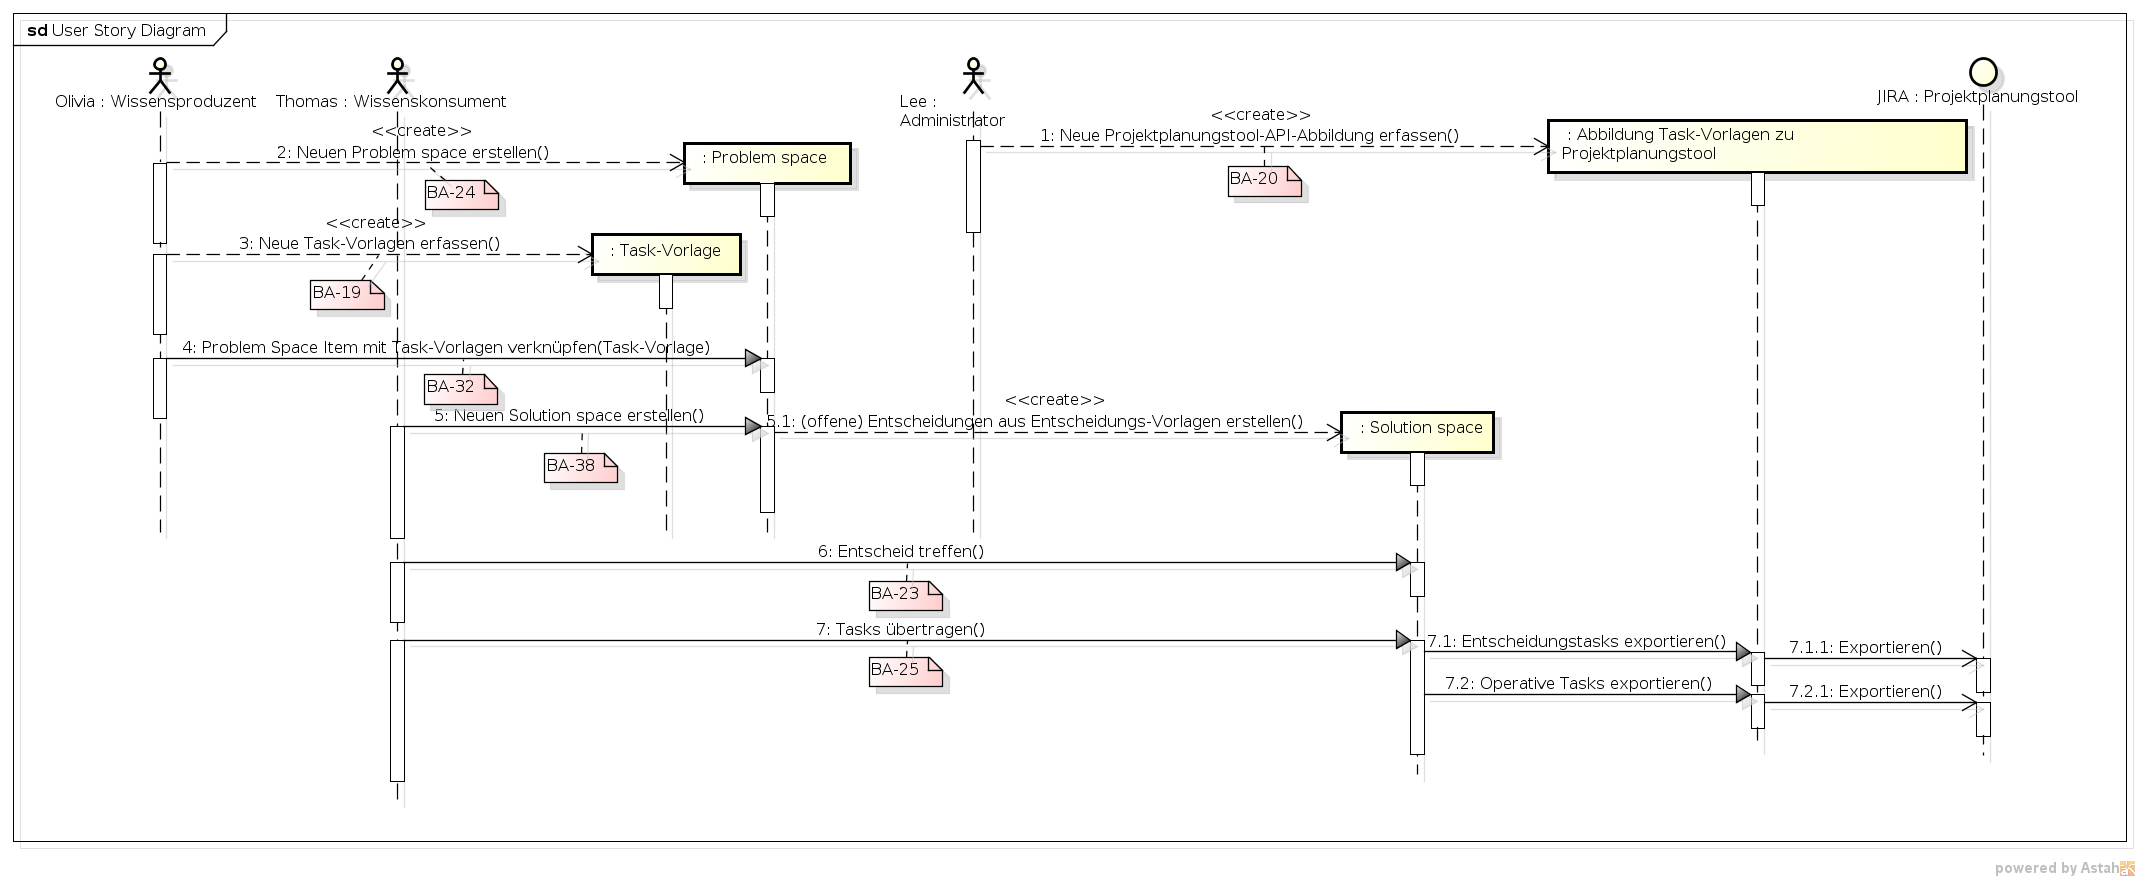
\includegraphics[width=0.95\linewidth]{media/diagrams/UserStoryDiagram.png}
				\centering
				\caption{Übergeordnete User Stories (inklusive \cdar)}
				\label{fig:UserStoryDiagram}
		\end{figure}
		
		Dabei repräsentieren die drei Aktore (Wissensproduzent, -konsument und Administrator) Personen wie in Abschnitt~\ref{userstoryDefinitions} beschrieben,
		der Business-Aktor (ganz rechts) repräsentiert ein beliebiges \ppt\ und die roten Kästchen referenzieren den dazugehörenden Issue im \eeppi-\ppt.
		Nachfolgend sind die Erklärungen für die aufgezeigten User Stories.
		Die User Stories sind jeweils im Format nach Mike Cohn\cite{rasmusson_agile_2012} beschrieben:
		\begin{quote}
			\textbf{As a} <type of user>,\newline
			\textbf{I want} <to perform some task>\newline
			\textbf{so that I can} <achieve some goal/benefit/value>.
		\end{quote}
	\end{landscape}

		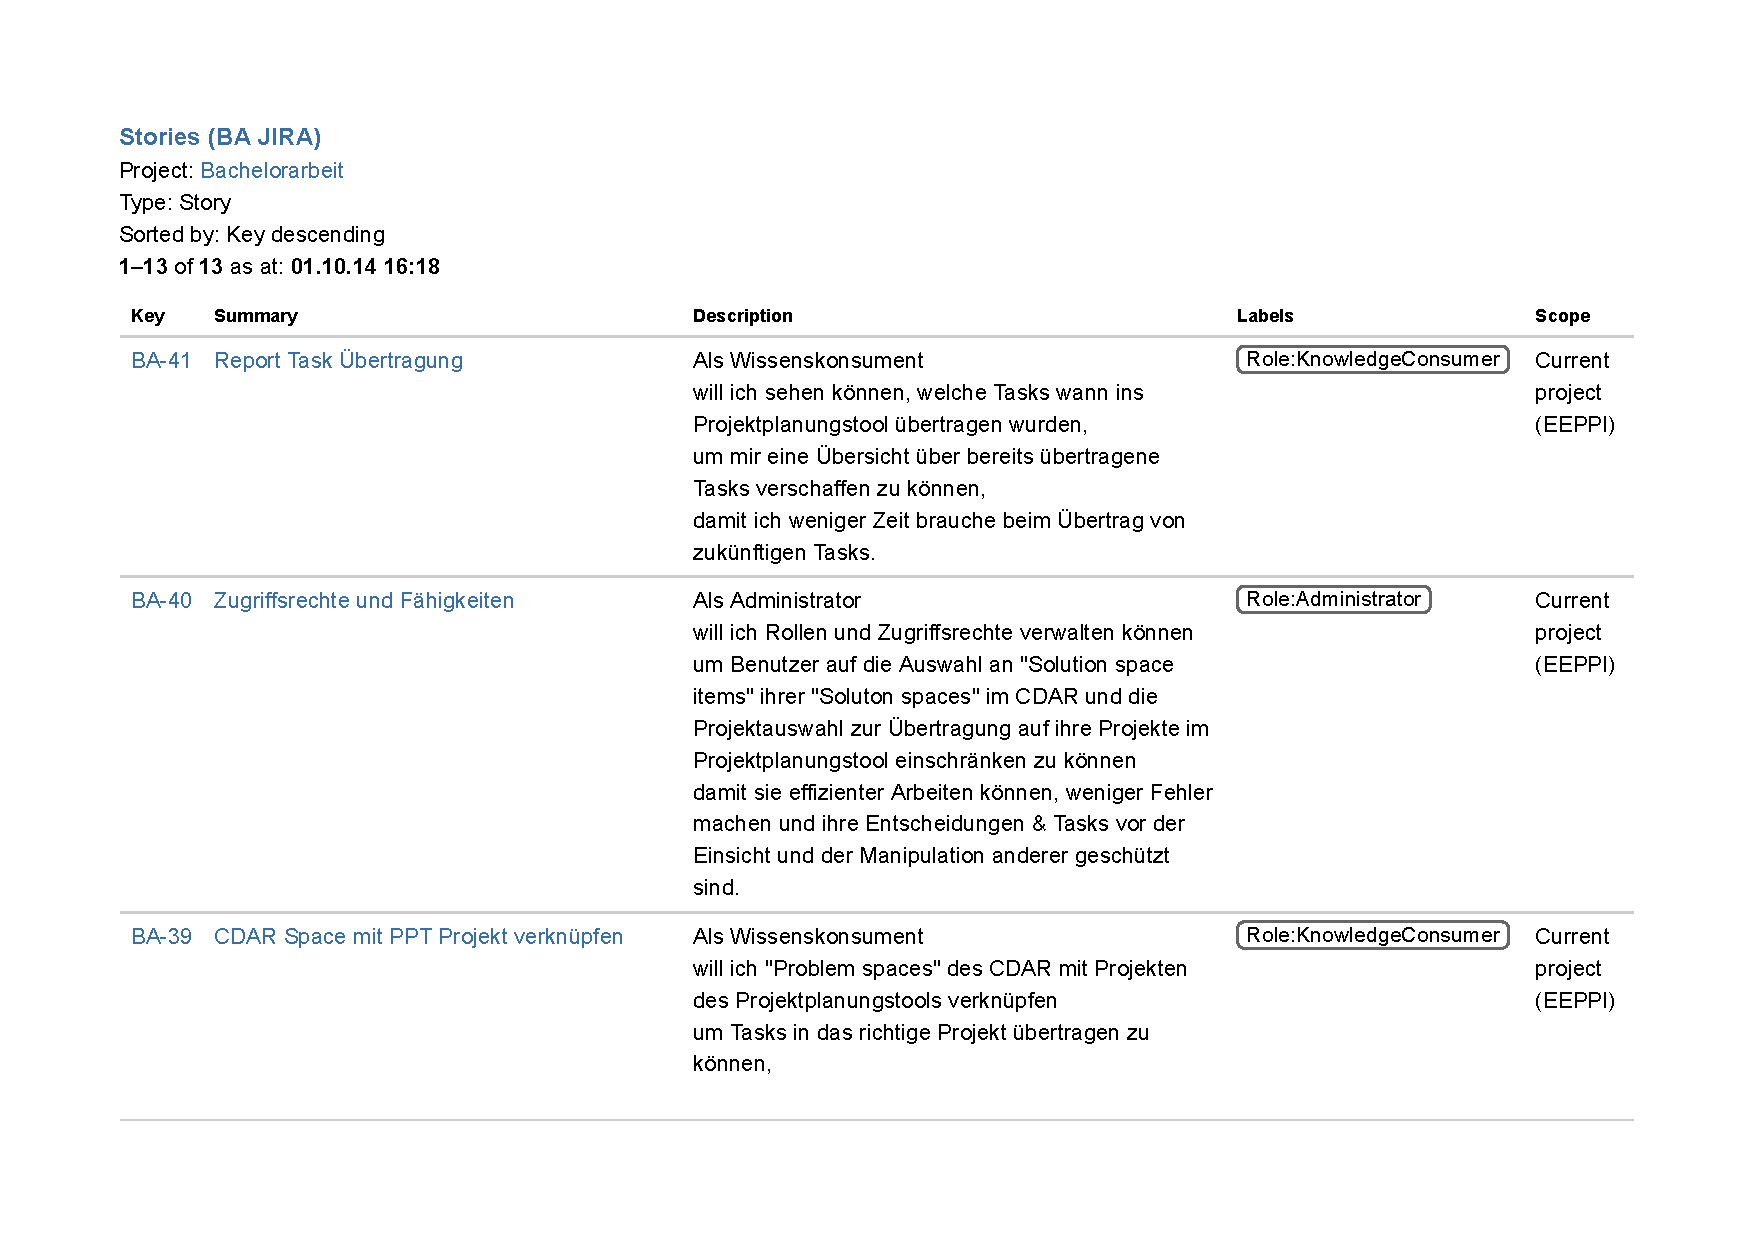
\includepdf[pages=-, pagecommand={}, scale=0.975, landscape=true]{requirements/media/documents/stories.pdf}